\documentclass[../main.tex]{subfiles}
\begin{document} \label{chapter_account}
In this chapter, we describe our implementation of the general pipeline described in section \ref{general_pipeline} and the achieved results. On one hand, we describe the birdsong dataset and the corresponding preprocessing techniques we used, as well the algorithms and packages used to implement formant trajectory extraction, Kernel Density Estimation, Variational Hidden Markov Models and Agglomerative Hierarchical Clustering, as described in chapters \ref{chapter_formants} and \ref{chapter_hmms}. On the other hand, we present the achieved relational structures (henceforth called phylo-acoustic trees) and other experiments performed over birdsong data.

\section{Implementation} \label{section_implementation}
We implemented a system capable of building phylo-acoustic trees automatically. The implementation runs in MATLAB 2015a and all the experiments were executed on a computer with an Intel i5-3317U CPU, 8.00 GB RAM, running Windows 8.1 64-bits. 
\par With respect to the data, we used the Animal Sound Archive bird vocalisation dataset, which contains 3686 birdsong recordings of more than 100 different bird species from all over Europe. We used the data for 82 bird species that had at least 15 seconds of birdsong recording each. All the recordings are in WAV format (i.e. uncompressed) and sampled at 22,500 Hz, for reasons that will become clearer when we present the formant trajectory extraction implementation. 

\subsection{Formant trajectory extraction} \label{section_impformants}
As reviewed in chapter \ref{chapter_formants}, the goal of formant trajectory extraction is to generate a vector $\V{F} = \{\V{f}_1, \V{f}_2, ..., \V{f}_W\}$ of formants $\V{f}_i$ in each signal frame. We now use the signal processing techniques described in section \ref{subsection_preproc}: a pre-emphasis filtering with $\alpha = 0.95$ is first applied to the birdsong recording, which is then segmented into frames of 40 ms with an overlap of 50\% \cite{Stowell2014}. Every frame is then convoluted with a Hamming window to avoid sharp-edged frames. 
\par The number of formants we estimate per window corresponds to the rule of thumb $N_f = f_s / 2000$, where $f_s$ is the sampling frequency of the recording. Since birdsong goes to frequencies as high as 10,000 Hz \cite{Marler2004}, and that we want to have 1 formant per thousand Hz, all the birdsong files must be sampled at 22,500 Hz. Furthermore, the order of the LPC model corresponds to the rule of thumb $p = 2N_f + 2$, i.e. we have 1 formant for every 2 roots, and let the model have an extra 2 roots to handle very low frequencies where large amounts of energy are contained, but are not resonances of the vocal tract \cite{Benesty}. 
\par Finally, the autocorrelation $\V{r}$ is estimated by using the Wiener-Khinchin Theorem and the rest of the formant trajectory extraction proceeds as outlined in chapter \ref{chapter_formants}, and summarised in algorithm \ref{alg_formants}. MATLAB contains an implementation of the Fast Fourier Transform algorithm and polynomial root solving algorithms. Furthermore, the Signal Processing Toolbox contains an implementation of the Levinson-Durbin recursion. These algorithms were assembled in a single, parametrised procedure to extract formants from recordings.

\begin{algorithm}
\begin{algorithmic}[1]
\Function{formants}{$\V{s}_i$, $f_s$, $N_f$}
\State $\V{S}$ = fft($\V{s}$)
\State $\V{R}$ = inv\_fft( $\V{S} \cdot \bar{\V{S}}$ )
\State $\V{a}$ = levinson($\V{r}, p$)
\State $\left[\V{r}, \theta\right]$ = roots($\V{a}$)
\State $\V{f}_i$ = $\theta \cdot \frac{f_s}{2\pi}$
\State $\V{b}_i$ = $-\frac{f_s}{4\pi}\log{\V{r}}$
\EndFunction
\caption{Formant extraction for a signal frame $\V{s}$.}\label{alg_formants}
\end{algorithmic}
\end{algorithm}

\par Once the formants for a given window have been calculated, all values $f_{i, j} < 500 Hz$ are filtered as noise \cite{Stowell2014}, and only the formants with a bandwidth narrower than 500 Hz are kept \cite{Mathworks2015}. However, not all of these formants are useful. Although we do not give a formal proof, in subsection \ref{section_choosing} we show that the individual trajectory corresponding to the first formant of every segment if the smoothest one. Characterising each recording by a single, unidimensional trajectory allows us to simplify the parametrisation and training of the statistical models discussed in chapter \ref{chapter_hmms}, hence trading complex features for a potentially more efficient and accurate statistical description.
\par Nevertheless, we still provide an implementation that extracts a specific number of formants. An example of the output produced for the first formant trajectory of a birdsong recording is shown in figure \ref{fig_traj}.

\begin{figure}[t]
\centering
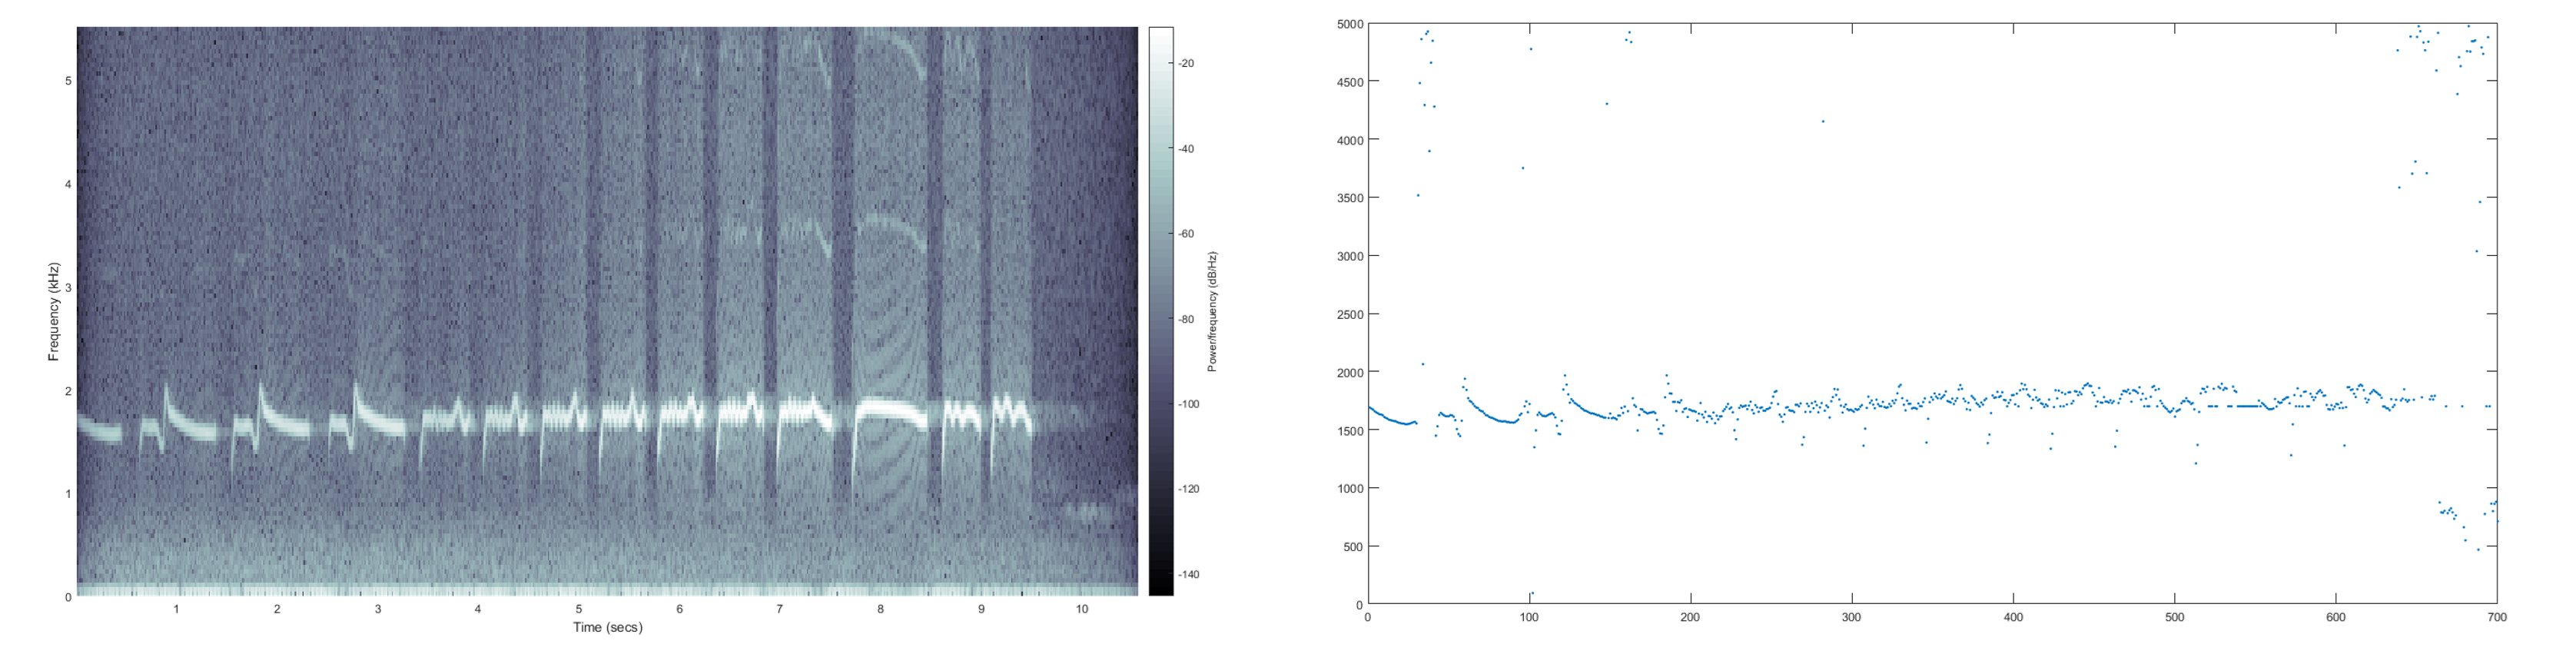
\includegraphics[width=\textwidth]{formant_traj}
\caption{To the right, the first formant trajectory extracted from a birdsong recording of the species \emph{Certhia brachydactyla}; to the left, the spectrogram corresponding to this recording. Note that the extracted trajectory corresponds with the bright patterns in the spectrogram, where present.}
\label{fig_traj}
\end{figure}

\subsection{Kernel Density Estimation and Hidden Markov Models} \label{section_imphmms}
In this section, we describe the implementations of Kernel Density Estimation and Variational Hidden Markov Models.
\par The function ksdensity is included in the MATLAB Statistics and Machine Learning Toolbox. It receives as input a vector of formants $\V{x}$ and an interval of points $\V{p}$ to evaluate the probability distribution at. For the case of univariate Gaussian kernels, it sets the bandwidth $h$ to a theoretical optimal, as discussed in section \ref{section_kde}. After estimating the probability distribution of each recording, all the distributions corresponding to the same species are averaged to obtain a single, characterising distribution per species. Figure \ref{fig_kdespecies} shows the result of this procedure for 5 different bird species in the ASA dataset.

\begin{figure}[t]
\centering
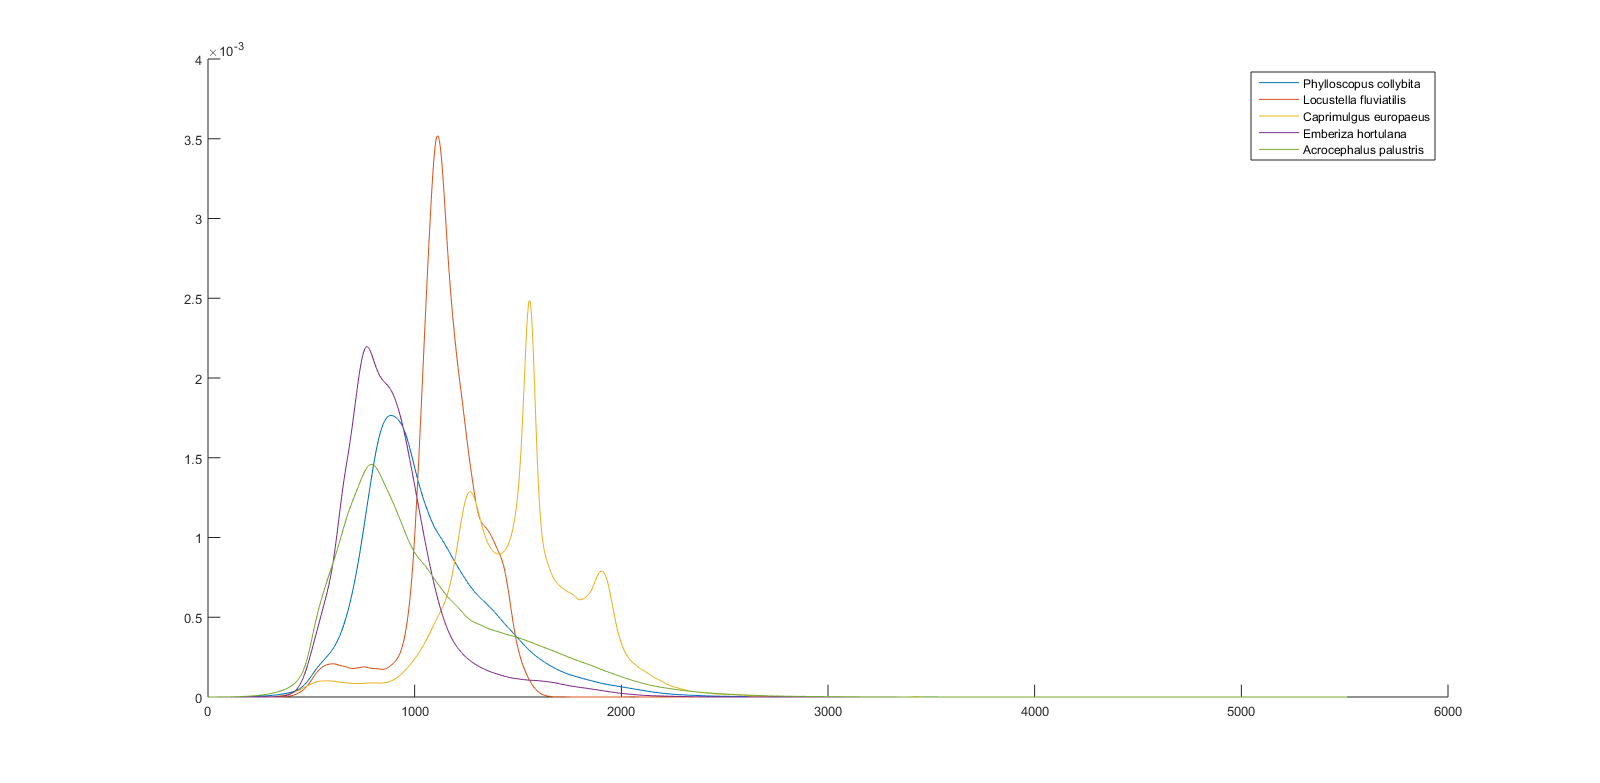
\includegraphics[width=\textwidth]{kdespecies}
\caption{Comparison of probability distributions generated by KDE for 5 different species. Despite having high probability in similar ranges of frequencies, their shapes are still distinguishable. }
\label{fig_kdespecies}
\end{figure}

\par Concerning Variational HMMs, we used the implementation of the Oxford Machine Learning Research Group, HMMBOX 4.1, which requires the NETLAB package. The former contains implementations of the tools required for a Bayesian treatment of HMMs, in particular: implementation of closed forms for the KL-divergence of the Normal, Dirichlet and Wishart distributions, variational inference training and sequence decoding. Furthermore, a routine that computes the occupancy of an HMM $\Omega_\lambda$ with respect to a sequence $\V{x}$ was also implemented. 
\par After computing the formant trajectories for each recording, the ones corresponding to a single species were concatenated and used as the training sequence for each HMM, i.e. we trained one HMM per species, and then computed their occupancy with respect to their respective training sequences. We used a Gaussian observation model for every HMM.

\subsection{Similarity matrices and Hierarchical Clustering}
The Hellinger distance and the Symmetric KL Divergence were implemented in MATLAB to compute distances between discrete distributions. These were used to compute the distance between each pair of densities obtained from the KDE procedure. In MATLAB, this can be done efficiently by means of the pdist function, a vectorised implementation that receives a metric and a matrix with observations as rows, and computes the distance between each pair of rows.
\par With respect to HMMs, similarity computation is performed in two different approaches: one consists in computing the Hellinger distance or the SKLD between each pair of emission models (Gaussian Mixture Models). The other approach consists in sorting the HMMs' states (so as to avoid the identifiability problem discussed in chapter \ref{chapter_hmms}), and then computing the distance between each pair of Dirichlet distributions from the transition model. This distance metric corresponds to the definition given in equation \ref{eq:hmmdist}.
\par Then, we used the distance matrices obtained from these procedures to generate phylo-acoustic trees using Agglomerative Hierarchical Clustering. The MATLAB Statistics and Machine Learning Toolbox contains routines to compute the three linkage procedures described in section \ref{section_hierarchical}. In particular, the function linkage receives a distance matrix and outputs a new matrix $\V{Z}$. The first two columns of $\V{Z}$ correspond to the identifiers of the merged clusters, and the third column displays the intergroup distance between the two clusters at time of merging. Additionally, the results of this stage can be evaluated by means of the cophenetic correlation coefficient, implemented in MATLAB via the cophenet function.
\par Finally, the dendrogram function was used to plot the clusters resulting from the linkage stage as a tree. Due to the monotonicity of agglomerative clustering, a dendrogram representation of the $\V{Z}$ is always available. 

\subsection{Conclusion} \label{section_5conclusion}
In this section, we described the implementation of the algorithms described in chapters  \ref{chapter_formants} and \ref{chapter_hmms}. A flowchart summarising these approaches is depicted in figure \ref{implementation_pipeline}. The results outcoming from each of these will be presented in section \ref{section_results}. 

\begin{figure}
\centering
\begin{tikzpicture}[node distance=2cm]
\node (start) [startstop] {Start};
\node (in1) [io, below of=start] {Animal Sound Archive dataset};
\node (pro1) [process, below of=in1] {Formant trajectory extraction};
\node (in2) [io, below of=pro1] {Formant trajectories};
\node (pro2) [process, below left=of in2] {KDE};
\node (pro2b) [process, below right=of in2] {Train HMM};
\node (pro3) [process, below = 2.5 cm of pro2] {Compute SKLD or Hellinger};
\node (pro3b) [process, below left=1 cm and -1.4 cm of pro2b] {SKLD/Hellinger between GMMs};
\node (pro3c) [process, below right=1 cm and -1.4 cm of pro2b] {Distance between Dirichlets};
\node (pro4) [process, below=7cm of in2] {Build relational structure};
\node (out1) [io, below=of pro4] {Relational structure};
\draw [arrow] (start) -- (in1);
\draw [arrow] (in1) -- (pro1);
\draw [arrow] (pro1) -- (in2);
\draw [arrow] (in2) -- (pro2);
\draw [arrow] (in2) -- (pro2b);
\draw [arrow] (pro2) -- (pro3);
\draw [arrow] (pro2b) -- (pro3b);
\draw [arrow] (pro2b) -- (pro3c);
\draw [arrow] (pro3) -- (pro4);
\draw [arrow] (pro3b) -- (pro4);
\draw [arrow] (pro3c) -- (pro4);
\draw [arrow] (pro4) -- (out1);
\end{tikzpicture}
\caption{A general pipeline to build relational structures.}
\label{implementation_pipeline}
\end{figure}

\section{Results} \label{section_results}
In section \ref{section_implementation}, we described implementation details concerning the algorithms and models described in chapters \ref{chapter_formants} and \ref{chapter_hmms}. In this section, we describe the results and experiments gathered from this implementation. We first show empirical evidence on why the first formant of a signal potentially gives the most structural information about formant trajectories than any other formant. This supports empirically our choice to train statistical models only over the trajectory of the first formant. 
\par Then, we present phylo-acoustic trees for each of the paths from the flowchart in figure \ref{implementation_pipeline}. We first provide a qualitative assessment of these results, and then proceed to show formally that this data analysis does exhibit a clear structure.

\subsection{Choosing the number of formants} \label{section_choosing}
In subsection \ref{section_impformants}, we briefly justified why choosing only the first non-zero formant (in ascending order) from each signal segment to train statistical models was reasonable. We now aim to give further evidence about this choice. Although providing a rigorous argument about this is outside of the scope of this project, we offer empirical evidence that strongly suggests that the F1 trajectory (the trajectory built using only the first formant of each segment of a signal) is the most structured one in average for our recordings. This allows us to train unidimensional models over the most structured sequence obtained from out dataset.
\par Consider a single recording with a $D$-formant trajectory $\V{F} = \{\V{f}_1, \V{f}_2, ..., \V{f}_W\}$, $\V{f}_i \in \mathbb{R}^D$. For a trajectory $\V{F}$, we define the consecutive formant window difference $\hat{\V{f}}$ as:
\begin{align*} 
\hat{\V{f}} = \sum_{i=2}^W \abs{\V{f}_{i} - \V{f}_{i-1}}
\end{align*}
\par Note that the larger any entry $\hat{\V{f}}_k$ is, the more scattered formant $k$ is along the frequency axis. Our hypothesis is that, if all individual formant trajectories F1, F2, ..., FD for a given recording were equally structured, then the vector $\hat{\V{f}}$ would tend to be uniform. Recall from section \ref{section_impformants} that we used a rule of thumb to find one formant every 1 kHz. The more the formants jump from one frequency band to another (i.e. the less structured they are), the larger the difference between consecutive windows becomes. Figure \ref{fig_choose} shows an example in which $\hat{\V{f}}_1$ is smaller than both, $\hat{\V{f}}_2$ and $\hat{\V{f}}_3$.

\begin{figure}[ht]
\centering
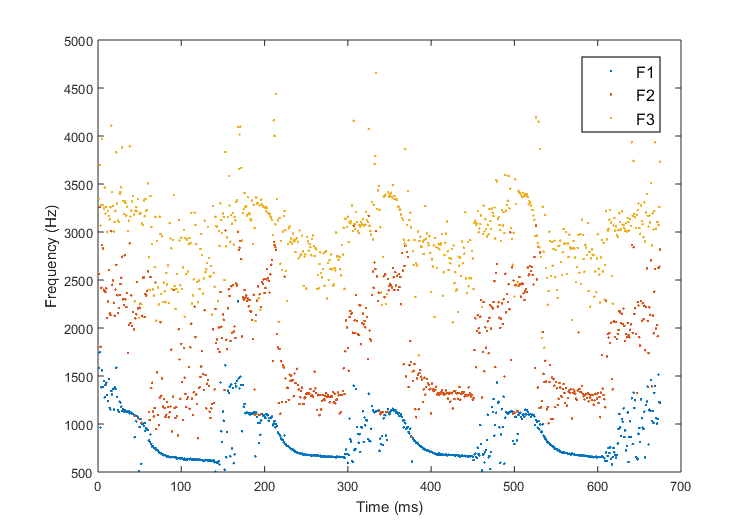
\includegraphics[width=\textwidth]{choose}
\caption{A formant trajectory where the first three formants F1 (blue), F2 (red), F3 (yellow) have been extracted from each frame. Note that F2 and F3, although not completely lacking a structure, look considerably less smooth than F1 over time.}
\label{fig_choose}
\end{figure}
\par Now consider the set of vectors:
\begin{align*}
\mathcal{C} = \left\{\frac{\hat{\V{f}}^{(1)}}{\hat{\V{f}}^{(1)}_1}, \frac{\hat{\V{f}}^{(2)}}{\hat{\V{f}}^{(2)}_1}, ..., \frac{\hat{\V{f}}^{(\abs{R})}}{\hat{\V{f}}^{(\abs{R})}_1}\right\}
\end{align*}
where $\abs{R}$ is number of birdsong recordings contained in our dataset. This set describes the consecutive difference vectors divided by the consecutive difference of the first formant, i.e. for each bird species, each vector describes how much more scattered the $k$-th formant is with respect to the first formant. For any scalar greater than 1, we conclude that formant $k$ is more scattered than F1 for that recording according to this measure. 
\par In this experiment, we first compute the formant trajectories with the first seven formants of every recording in our dataset, and use them to provide evidence of the comparatively less structured shape of formants greater than F1. To this end, consider the quantity:
\begin{align*}
f'_{i, j} = \frac{1}{\abs{\mathcal{R}}}\sum_{r \in \mathcal{R}} \mathbb{I}(\hat{\V{f}}^{(r)}_i < \hat{\V{f}}^{(r)}_j)
\end{align*}
i.e. the proportion of recordings in which the individual trajectory for formant $i$ had more structure than the one for formant $j$. We give the quantities $\mu(\mathcal{C})$, i.e. the average of the set $\mathcal{C}$, and $f'_{i, 1}, \forall j > 1$ in table  \ref{table_choose}.
\begin{table}[ht]
\centering
\begin{tabular}{r|r|r|r|r|r|r|r} 
 \textbf{Qty} &\textbf{F1} &  \textbf{F2}&  \textbf{F3}&  \textbf{F4}&  \textbf{F5}&  \textbf{F6}&  \textbf{F7}\\
 \hline
 $\mu(\mathcal{C})$ & 1.0000  &  2.4295  &  2.6233  &  2.9560  &  3.2443  &  3.5412  &  3.9243 \\
 $f'_{i, 1}$ & 0 & 0.0794 & 0.0565 & 0.0199 & 0.0024 & 0 & 0
\end{tabular}
\caption{The first row of this table describes how much more scattered an individual formant trajectory is with respect to the first formant, F1. The second row describes the proportion of recordings that have more structure than F1 in the whole dataset according to the consecutive formant difference metric.}\label{table_choose}
\end{table}
\par According to this data, all individual formant trajectories were at least twice as scattered than F1 in average, and only did less than 8\% of the recordings ever have a formant trajectory with more structure than F1 according to this measure. Despite not being a formal proof, this experiment strongly suggests that F1 is the a suitable choice for training a statistical model with unidimensional data.

\subsection{Generating phylo-acoustic trees} \label{subsection_phylo}
In this section, we present the final output of the implementation pipelines discussed throughout the chapter. We have generated 6 phylo-acoustic trees in accordance with the flowchart from figure \ref{implementation_pipeline}, which are:
\begin{itemize}
\item Symmetric KL Divergence over non-parametric distributions generated via KDE.
\item Hellinger distance over non-parametric distributions generated via KDE.
\item Symmetric KL Divergence over Gaussian Mixture Models trained as emission models for a Hidden Markov Model.
\item Hellinger distance over Gaussian Mixture Models trained as emission models for a Hidden Markov Model.
\item Symmetric KL Divergence over the Dirichlet distributions associated to the transition models of our Hidden Markov Models.
\item Occupancy-weighted Symmetric KL Divergence (as described in \ref{subsection_hmmsim}) over the Dirichlet distributions associated to the transition models of our Hidden Markov Models.
\end{itemize}
\par Full-size figures of each phylo-acoustic tree are offered in appendix \ref{app_phylo}. Brown marks have been added to each figure whenever more than 40\% of a cluster consisted of species from the same genus (i.e. they share the first word in their scientific names). 
\par These trees can be assessed in several ways - choosing to mark clusters whose species share an ancestor is just one of them. The versatility of this approach suggests that, rather than proving that facts from Zoology extend to Acoustic Analysis, we can change the focus and contribute to these facts by showing empirical evidence about relationships that could be unexpected from their point of view.
\par This key point was briefly discussed in chapter \ref{chapter_soa}, when we argued that birds sharing common ancestors need not necessarily share birdsong traits in the future. Birdsong is not uniquely determined by genes, instead it often suffers modifications that are due to mating advantage and adaptation to new environments. For this reason, relations unveiled in phylo-acoustic trees could also be linked to migration patterns and, more generally, geolocalisation.
\par Nevertheless, one of the most important conclusions we aim to draw from these trees is that their structure is no coincidence. We address this in subsection \ref{subsection_null}.

\subsection{Phylo-acoustic trees are not a coincidental} \label{subsection_null}
In subsection \ref{subsection_phylo}, we presented 6 examples of phylo-acoustic trees generated from instantiations of the more general pipeline proposed in chapter \ref{chapter_soa}. A qualitative assessment of these trees does show clusters with birds from the same genus, i.e. suggesting that some birds with common ancestors still have similar traits in their songs. However, we also suggested that other relations, such as co-existence in geographical areas could also lead to convergence in birdsong, hence making apparently unrelated species be close in the phylo-acoustric dendrograms.
\par In this subsection, we aim to show that the structure unveiled by these phylo-acoustic trees is not coincidental. To achieve this, we aim to disprove the null hypothesis:
\begin{align*}
H_0 = \text{there is no relationship between the species in a phylo-acoustic tree.}
\end{align*}
\par If this hypothesis is true, then randomly generated data has the same structure as any of these trees. To generate such data, we sample random formant trajectories from the uniform distribution $\mathcal{U}(f_{min}, f_{max})$, where the boundaries of the distribution correspond to the minimum and maximum formant seen in any species in the dataset. This key step guarantees that the structure present in the real phylo-acoustic trees is not only due to the range of frequencies in formant trajectories.
\par After generating as many formant trajectories as bird species, we follow each of the pipelines described in subsection \ref{subsection_phylo} and generate new ``phylo-acoustic trees'' for each of them. The resulting trees are shown in appendix \ref{app_phylo}.
\par We compare each pair of trees generated using the same technique by plotting how the number of clusters changes through time. When there is real structure in data, clusters are tight and well separated from each other. This implies the distance between clusters becomes larger as smaller clusters merge. This maps visually to long branches in a dendrogram. 
\par On the other hand, when there is no real structure in data, objects tend to be similar distances apart from each other (they are uniformly scattered in space). When a new cluster is formed, linkage methods tend to change very little the distances between the original clusters, since they were very similar before merging. This translates into clusters that have a short life.
\par The dendrogram is not a representation suitable to compare structured and non-structured data in parallel. Instead, we opt to generate a plot where we can compare the evolution of both, real and random trees, at the same time. In particular, we choose to plot the lifetime (from 0 up to the lifetime of the longest-living cluster) versus the number of clusters in each tree. The plots corresponding to each pipeline can also be found in appendix \ref{app_phylo}.
\par In all six cases we obtain similar results. The red curves depicting the random statistical models go down very quickly due to clusters that live too little, as opposed to the blue lines (real data), which live many orders of magnitude longer.
\par These findings are strong arguments to reject the null hypothesis and hence conclude that real data does exhibit real structure.
\section{Conclusion}
In this chapter, we discussed the implementation details for specific pipelines that output phylo-acoustic trees. In particular, we presented guidelines to make a full implementation of these pipelines using the algorithms and techniques described in chapter \ref{chapter_formants} and \ref{chapter_hmms}.
\par The final chapter provides further discussion on the results obtained, and highlights areas that could lead to future work.

\end{document}